\section{The Step Potential}
\subsection{Energy Above the Barrier}\label{energy_above_barrier}

We now begin our study of \textbf{scattering states}. These are energy eigenstates that cannot be normalized:

\begin{frameddefn}[Scattering states]
    A scattering state is an energy eigenstate that cannot be normalized.
\end{frameddefn}

Similarly to the plane waves we considered earlier, these do not represent physical states of a particle. Instead, we must consider superpositions of these states for them to have physical meaning.

We begin by considering the \textbf{step potential} $$V(x)=\begin{cases}0 & x<0 \\ V_0 & x\geq 0\end{cases}$$There are two cases: $E>V_0$ and $E<V_0$. In both cases, the wavefunction extends infinitely to the left and is non-normalizable. In this section, we consider the case $E>V_0$, as depicted in Figure \ref{step_e_bigger}.

\begin{figure}
    \centering
    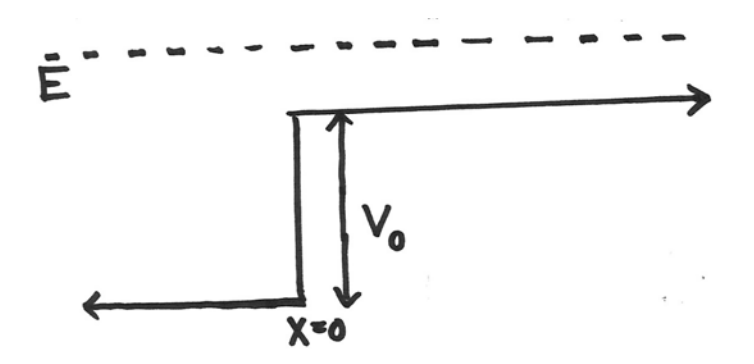
\includegraphics[width=0.5\linewidth]{resources/images/step_e_bigger.png}
    \caption{A sketch of the step potential for $E>V_0$.}
    \label{step_e_bigger}
\end{figure}

To find $\psi(x)$, we imagine a physical process in which a wave $Ae^{ikx}$ is incident on the step from the left. We would expect a reflected wave $Be^{-ikx}$ moving to the left from the step and a transmitted wave $Ce^{i\bar{k}x}$ moving to the right: $$\psi(x)=\begin{cases}Ae^{ikx}+Be^{-ikx}&x<0 \\ Ce^{i\bar{k}x}&x>0\end{cases}$$We can obtain the wavenumbers $k$ and $\bar{k}$ via the Schrödinger equation: $$k^2=\frac{2mE}{\hbar^2},\quad\bar{k}^2=\frac{2m(E-V_0)}{\hbar^2}.$$Furthermore, both $\psi$ and $\psi'$ must be continuous at $x=0$; these boundary conditions constrain the values of $A$, $B$, and $C$. Continuity of $\psi$ gives $A+B=C$, and continuity of $\psi'$ gives $ikA-ikB=i\bar{k}C$. Rearranging, $A-B=\frac{\bar{k}}{k}C$. Solving for $B$ and $C$ in terms of $A$, we get $$\frac{B}{A}=\frac{k-\bar{k}}{k+\bar{k}},\quad\frac{C}{A}=\frac{2k}{k+\bar{k}}.$$This is the best we can do; the value of the independent variable $A$ can be thought of as the \textit{input}, since it defines the amplitude of the incoming wave. Mathematically, it represents a normalization factor.

In the limit as $E\to V_0$, we have $\bar{k}\to 0$, so $B=A$ and $C=2A$. Then the solution is $$\psi(x)=\begin{cases}2A\cos(kx)&x<0 \\ 2A&x>0\end{cases}$$This wavefunction is shown in Figure \ref{e_bigger_v_wavefunction}.

\begin{figure}[H]
    \centering
    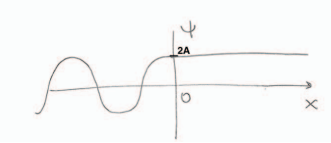
\includegraphics[width=0.5\linewidth]{resources/images/e_bigger_v_wavefunction.png}
    \caption{A sketch of the wavefunction in the limit as $E\to V_0$.}
    \label{e_bigger_v_wavefunction}
\end{figure}

We can obtain further insight by evaluating the probability current just to the left and the right of the step. Recall from Theorem \ref{current_conservation_thm} that the probability current $J$ for a wavefunction $\psi$ is $$J=\frac{\hbar}{m}\operatorname{Im}(\psi^*\frac{\partial\psi}{\partial x}).$$A short calculation shows that the current $J_L$ to the left of the step is $$J_L=\frac{\hbar k}{m}(|A|^2-|B|^2)=J_A-J_B,$$where $J_A=\frac{\hbar k}{m}|A|^2$ and $J_B=\frac{\hbar k}{m}|B|^2$. Note that there is no interference between the incident and reflected waves; the total current to the left of the step is simply the incident wave current minus the reflected wave current. Similarly, the current $J_R$ to the right of the step is $$J_R=\frac{\hbar \bar{k}}{m}|C|^2=J_C.$$Note that both $J_L$ and $J_R$ are time-independent. Thus, current conservation requires $J_L=J_R$ -- the current must be independent of position. We check that \begin{align*}J_L &=\frac{\hbar k}{m}(|A|^2-|B|^2) \\ &=\frac{\hbar k}{m}(1-(\frac{k-\bar{k}}{k+\bar{k}})^2)|A|^2 \\ &= \frac{\hbar k}{m}(\frac{4k\bar{k}}{(k+\bar{k})^2})|A|^2 \\ &=\frac{\hbar \bar{k}}{m}\frac{4k^2}{(k+\bar{k})^2}|A|^2=\frac{\hbar k}{m}|C|^2=J_R.\end{align*}

\subsection{Reflection and Transmission Coefficients}\label{reflection_transmission_coefficients}

However, since the incident and reflected waves do not interfere, current conservation gives us $J_A-J_B=J_C$. Rearranging, $$1=\frac{J_B}{J_A}+\frac{J_C}{J_A}.$$We define the \textbf{reflection coefficient} $R$ as the ratio of the probability flux due to the reflected wave to that of the incident wave: $$R=\frac{J_B}{J_A}=\frac{|B|^2}{|A|^2}=(\frac{k-\bar{k}}{k+\bar{k}})^2\leq 1.$$Similarly, we define the \textbf{transmission coefficient} $T$ as the ratio of the probability flux due to the transmitted wave to that of the incident wave: $$T=\frac{J_C}{J_A}=\frac{\bar{k}}{k}\frac{|C|^2}{|A|^2}=\frac{\bar{k}}{k}\frac{4k^2}{(k+\bar{k})^2}=\frac{4k\bar{k}}{(k+k^2)}.$$We therefore have $$R+T=1.$$Note that the wavelengths to the left and right of the step are different, so $T\neq \frac{|C|^2}{|A|^2}$.

Recall that for $E=V_0$ we have $\bar{k}=0$. Then we have full reflection: $R=1$ and $T=0$. Indeed, the probability current associated with the constant wavefunction that exists for positive $x$ is zero.

\subsection{Energy Below the Barrier}\label{e_less_v_step}

We now consider the case when $E<V_0$, as depicted in Figure \ref{step_e_smaller}.

\begin{figure}
    \centering
    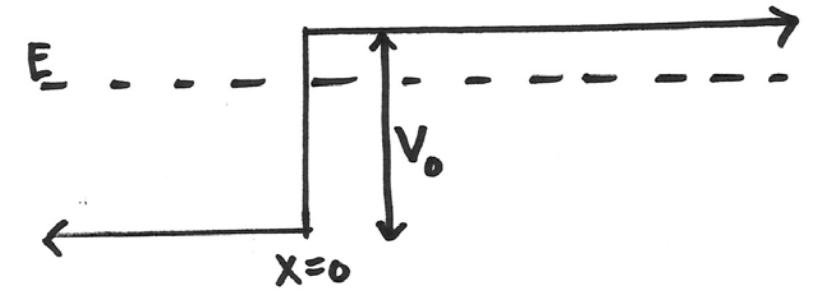
\includegraphics[width=0.5\linewidth]{resources/images/step_e_smaller.png}
    \caption{A sketch of the step potential for $E<V_0$.}
    \label{step_e_smaller}
\end{figure}

Now the region $x>0$ is classically forbidden. Let us try to solve for the energy eigenstate without redoing all the work we have already done in finding $B$ and $C$ in terms of $A$. Note that for $x<0$, the solution is unchanged and we still have $$\psi(x)=Ae^{ikx}+Be^{-ikx},\quad x<0$$ for $k^2=\frac{2mE}{\hbar^2}$. On the other hand, for $x>0$, the earlier solution $\psi(x)=C e^{i\bar{k}x}$ should become a decaying exponential $\psi(x)=C e^{-\kappa x}$ for $\kappa^2=\frac{2m(V_0-E)}{\hbar^2}$. Note that the former becomes the latter upon replacing $\bar{k}$ with $i\kappa$.

Therefore, we can simply perform this replacement in our earlier expressions for $B/A$ and $C/A$. In particular, we have $$\frac{B}{A}=\frac{k-i\kappa}{k+i\kappa}=\frac{i(k-i\kappa)}{i(k+i\kappa)}=-\frac{\kappa+ik}{\kappa-ik}=-e^{2i\delta(E)}$$with $$\delta(E)=\tan^{-1}(\frac{k}{\kappa})=\tan^{-1}(\sqrt{\frac{E}{V_0-E}}).$$Since the magnitude of $A$ is equal to the magnitude of $B$, we have $J_A=J_B$ and $J_C=0$. Thus, $T=0$ and $R=1$. As noted above, the ratio $\frac{B}{A}$ is a pure phase, and $\delta(E)\to 0$ as $E\to 0$. Note that $\delta(E)$ is positive and does not exceed $\pi/2$. A sketch of $\delta(E)$ is shown in Figure \ref{delta_step}.

\begin{figure}
    \centering
    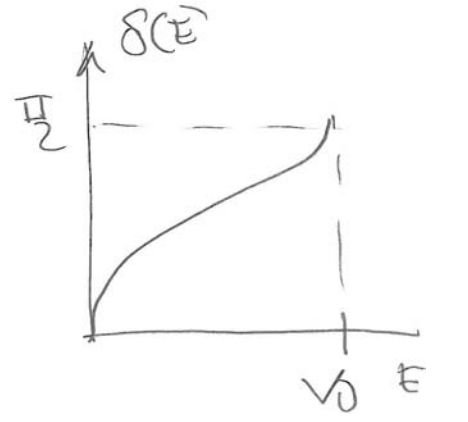
\includegraphics[width=0.5\linewidth]{resources/images/delta_step.png}
    \caption{A graph of $\delta(E)=\tan^{-1}(\sqrt{\frac{E}{V_0-E}})$.}
    \label{delta_step}
\end{figure}

The total wavefunction is $$\psi(x)=\begin{cases}Ae^{ikx}-Ae^{2i\delta(E)}e^{-ikx}&x<0 \\ Ce^{-\kappa x} & x>0\end{cases}$$For $x<0$, the wavefunction takes an interesting form: \begin{align*}\psi(x)&=Ae^{i\delta(E)}(e^{kx-\delta(E)}-e^{-i(kx-\delta(E))})\\ &= 2iAe^{i\delta(E)}\sin(kx-\delta(E)).\end{align*}Thus, the probability density is $$|\psi|^2=4A^2\sin^2(kx-\delta(E)).$$The point $x_0=\frac{\delta(E)}{k}>0$ in Figure \ref{step_e_smaller_wavefunction} is the point in the classically forbidden region where the extrapolation of the allowed-region solution would vanish. Of course, the probability density in the forbidden region is actually a decaying exponential. 

\begin{figure}[H]
    \centering
    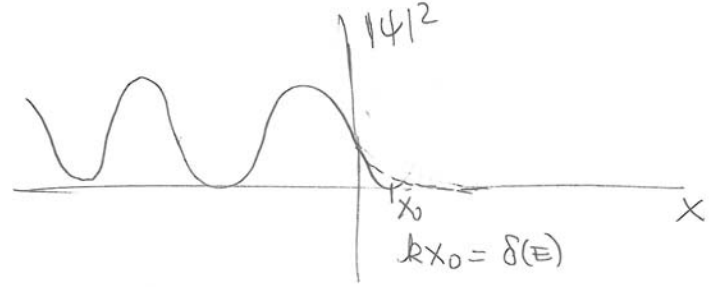
\includegraphics[width=0.5\linewidth]{resources/images/step_e_smaller_wavefunction.png}
    \caption{A sketch of the probability amplitude in the allowed and forbidden regions. At $x_0$, the forbidden region wavefunction is $0$, but the actual wavefunction is nonzero.}
    \label{step_e_smaller_wavefunction}
\end{figure}
For future use, we write the derivative of the phase $\delta(E)$: $$\delta'(E)=\frac{1}{2}\sqrt{\frac{1}{E(V_0-E)}}.$$This derivative becomes infinite for both $E\to 0$ and $E\to V_0$.

\subsection{Particle in the Forbidden Region}\label{particle_in_forbidden_region}

The fact that the wavefunction is nonzero in the forbidden region seems like it could lead to problems. Note that it would be contradictory if the observer could make both of the following two statements.

\begin{enumerate}
    \item The particle is located in the forbidden region.
    \item The particle has energy less than $V_0$. 
\end{enumerate}

If both statements were to hold simultaneously, the particle would have to have negative kinetic energy, which is impossible. How can we resolve this apparent contradiction? By invoking the uncertainty principle from Section \ref{widths_uncertainties}.

First note that in the forbidden region, the particle is governed by an exponentially decaying wavefunction of order $e^{-\kappa x}$. This implies that the particle penetrates a distance of approximately $\frac{1}{\kappa}$, where $$\kappa^2=\frac{2m(V_0-E)}{\hbar^2}.$$To be sure the particle is in the forbidden region, its position uncertainty $\Delta x$ must be smaller than the penetration depth: $$\Delta x\leq \frac{1}{\kappa}.$$By the uncertainty principle, the particle must have some momentum uncertainty $$\Delta p\geq \frac{\hbar}{\Delta x}\geq\hbar\kappa.$$Now there must be some uncertainty in kinetic energy $$\Delta KE=\frac{(\Delta p)^2}{2m}\geq \frac{\hbar^2\kappa^2}{2m}=V_0-E.$$Thus, given the first statement above, the second statement cannot be made! The very act of observing the particle in the forbidden region creates just enough uncertainty in the kinetic energy to make the total energy $V_0$. 

\section{Wavepackets on the Step Potential}

\subsection{Wavepackets with Energy Above the Barrier}\label{wavepackets_energy_above_barrier}

We now consider the physical states. As we've seen with the free particle in Section \ref{free_particle}, the stationary states are not normalizable. Instead, physical states are represented by wavepackets built from an infinite superposition of eigenstates. In this section, we will consider wavepackets built from energy eigenstates with $E>V_0$, or equivalently, $k^2>\hat{k}^2$, where $$k^2=\frac{2mE}{\hbar^2}>\frac{2mV_0}{\hbar^2}=\hat{k}^2.$$To begin with, we write the energy eigenstates including the time dependence. Let the wave be incident on the barrier at $t=0$. Setting $A=1$, we have $$\Psi(x,t)=\begin{cases}(e^{ikx}+\frac{k-\bar{k}}{k+\bar{k}}e^{-ikx})e^{-iE(k)t/\hbar} & x<0 \\ \frac{2k}{k+\bar{k}}e^{i\bar{k}x}e^{-iE(k)t/\hbar} & x>0\end{cases}$$We can form a superposition of these solutions by multiplying by a function $f(k)$ and integrating over $k$: 
$$\Psi(x,t)=\begin{cases}\int_{\hat{k}}^\infty dk\,f(k)(e^{ikx}+\frac{k-\bar{k}}{k+\bar{k}}e^{-ikx})e^{-iE(k)t/\hbar} & x<0 \\ \int_{\hat{k}}^\infty dk\,f(k)\frac{2k}{k+\bar{k}}e^{i\bar{k}x}e^{-iE(k)t/\hbar} & x>0\end{cases}$$
Here $f(k)$ is a real function of $k$ that is essentially zero except for a narrow peak at $k=k_0$. Note that we have only included momentum components with energy greater than $V_0$ by setting the lower bound of the integral to $\hat{k}$. The integral only ranges over positive $k$ because only in that case are the incident $e^{ikx}$ waves moving to the right. Since $\Psi$ is the superposition of eigenstates multiplied by a number $f(k)$, it is guaranteed to be a solution of the Schrödinger equation.

We can split the solution into incident, reflected, and transmitted waves: $$\Psi(x,t)=\begin{cases}\Psi_{inc}(x,t)+\Psi_{ref}(x,t) & x<0 \\ \Psi_{trans}(x,t) & x>0\end{cases}$$Of course, both $\Psi_{inc}$ and $\Psi_{ref}$ exist only for negative $x$, while $\Psi_{trans}$ exists only for positive $x$. We then have \begin{align*}\Psi_{inc}(x<0,t)&=\int_{\hat{k}}^\infty dk\,f(k)e^{ikx}e^{-iE(k)t/\hbar}, \\ \Psi_{ref}(x<0,t)&=\int_{\hat{k}}^\infty dk\,f(k)\frac{k-\bar{k}}{k+\bar{k}}e^{-ikx}e^{-iE(k)t/\hbar}, \\ \Psi_{trans}(x>0,t)&=\int_{\hat{k}}^\infty dk\,f(k)\frac{2k}{k+\bar{k}}e^{i\bar{k}x}e^{-iE(k)t/\hbar}.\end{align*}How does the peak of $\Psi_{inc}(x,t)$ move? To answer this question, we use the stationary phase approximation. Recall from Theorem \ref{principle_stationary_phase} that the main contribution to the integral occurs when the total phase in the integrand is stationary for $k\approx k_0$: $$\frac{d}{dk}(kx-\frac{\hbar^2k^2}{2m}\frac{t}{\hbar})\bigg|_{k_0}=0\implies x-\frac{\hbar k_0}{m}t=0.$$This is the relation between $t$ and $x$ satisfied by the peak of $\Psi_{inc}$. It describes a peak moving with constant positive velocity $\frac{\hbar k_0}{m}>0$. Since $\Psi_{inc}(x,t)$ requires that $x<0$, we only get a peak for $t<0$. For positive $t$, the stationary phase condition cannot be satisfied for any $x<0$, so $\Psi_{inc}(x,t)$ becomes negligible.

Now consider $\Psi_{ref}(x,t)$. This time, the stationary phase condition gives $$\frac{d}{dk}(-kx-\frac{\hbar^2 k^2}{2m}\frac{t}{\hbar})\bigg|_{k_0}=0\implies x+\frac{\hbar k_0}{m}t=0.$$This relation represents a peak moving with constant negative velocity $\frac{-\hbar k_0}{m}$. Since $\Psi_{ref}(x,t)$ requires that $x<0$, we only get a peak for $t>0$. This is intuitive, since the wave only reflects at $t=0$. For negative $t$, the stationary phase condition cannot be satisfied for any $x>0$, so $\Psi_{ref}(x,t)$ is negligible.

Finally, we consider $\Psi_{trans}(x,t)$. We have $$\frac{d}{dk}(\bar{k}x-\frac{\hbar^2k^2}{2m}\frac{t}{\hbar})\bigg|_{k_0}=0\implies \frac{d\bar{k}}{dk}\bigg|_{k_0}x-\frac{\hbar k_0}{m}t=0.$$From implicit differentiation using $\bar{k}^2=k^2-\frac{2mV_0}{\hbar^2}$, we know that $\frac{d\bar{k}}{dk}=\frac{k}{\bar{k}}$. Thus, we have $$\frac{k_0}{\bar{k}}x-\frac{\hbar k_0}{m}t=0\implies x=\frac{\hbar\bar{k}}{m}t.$$This relation represents a peak moving with constant positive velocity $\frac{\hbar\bar{k}}{m}$. Since $\Psi_{trans}(x,t)$ requires that $x>0$, we only get a peak for $t>0$. Again, this is intuitive, since the wave is only transmitted at $t=0$. For negative $t$, the stationary phase condition cannot be satisfied for any $x>0$, so $\Psi_{trans}(x,t)$ is negligible. 

\begin{framedrmk*}[Summary]
    For large negative times, $\Psi_{inc}$ dominates and both $\Psi_{ref}$ and $\Psi_{trans}$ are very small. For large positive times, both $\Psi_{ref}$ and $\Psi_{trans}$ dominate and $\Psi_{inc}$ is very small. These solutions are shown in Figure \ref{step_potential_solution_sketch}. For times close to $t=0$, all three waves exist and together describe the complex collision process.
\end{framedrmk*}

\begin{figure}[H]
    \centering
    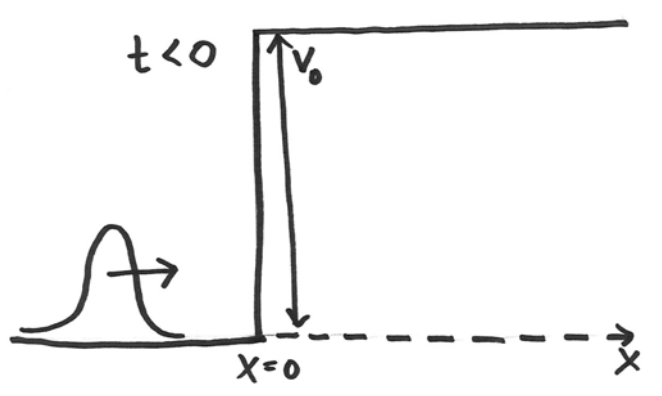
\includegraphics[width=0.4\linewidth]{resources/images/negative_t_step.png}
    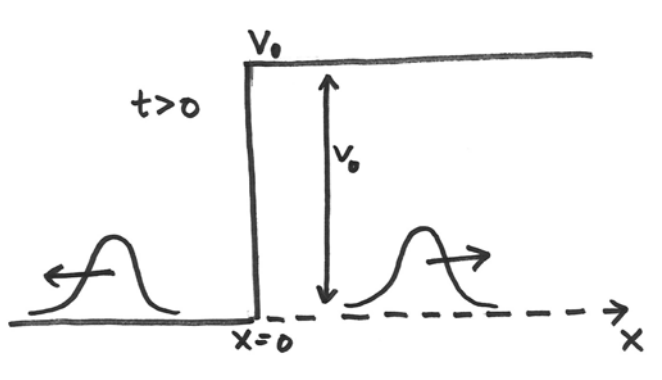
\includegraphics[width=0.45\linewidth]{resources/images/positive_t_step.png}
    \caption{A sketch of the behavior of the wavefunction for negative $t$ (left) and positive $t$ (right). Notice the incident, reflected, and transmitted wavepackets.}
    \label{step_potential_solution_sketch}
\end{figure}

\subsection{Wavepackets with Energy Below the Barrier}\label{wavepackets_energy_below_barrier}

We now consider a wavepacket built from eigenstates with energies $E<V_0$. Recall that in this situation $B/A=B=-e^{2i\delta(E)}$. Therefore, we have \begin{align*}\Psi_{inc}(x<0,t)&=\int_0^{\hat{k}} dk\,f(k)e^{ikx}e^{-iE(k)t/\hbar}, \\ \Psi_{ref}(x<0,t)&=-\int_0^{\hat{k}}dk\,f(k)e^{-ikx}e^{2i\delta(E)}e^{-iE(k)t/\hbar}.\end{align*}Note that the transmitted wave simply decays exponentially. However, the reflected wave is quite interesting. Using Theorem \ref{principle_stationary_phase} again, we have $$\frac{d}{dk}(2\delta(E)-kx-\frac{Et}{\hbar})\bigg|_{k_0}=0\implies2\delta'(E(k_0))\frac{\hbar^2k_0}{m}-x-\frac{\hbar k_0 t}{m}=0.$$Rearranging, we see that $$x=-\frac{\hbar k_0}{m}(t-2\hbar\delta'(E(k_0))).$$This represents a peak moving with constant negative velocity $-\frac{\hbar k_0}{m}<0$. However, there is also a \textbf{time delay} $\Delta t=2\hbar\delta'(E(k_0))$. Since the reflected wave is only defined for $x<0$, the peak does not begin to move until $t>2\hbar\delta'(E(k_0))$. We plotted $\delta(E)$ in Figure \ref{delta_step} and saw that its derivative diverges as $E$ approaches $0$ or $V_0$. Thus, the time delay is largest for wavepackets with very little energy or those with energy close to $V_0$.

\begin{framedrmk*}[Scattering theory]
    In scattering theory, physicists use this property of time delay to learn about unknown potentials by measuring the amount of time it takes for the reflected wave to begin moving. We will explore scattering theory in the next chapter.
\end{framedrmk*}

\section{Waves on the Finite Square Well}

\subsection{Reflection and Transmission Coefficients}\label{reflection_transmission_coefficients}

In Section \ref{finite_square_well}, we found the bound states of the finite square well potential $$V(x)=\begin{cases}0 & |x|>a \\ -V_0 & |x|<a\end{cases}$$

We now consider a scattering eigenstate with $E>0$ that represents an incoming wavefunction $Ae^{ikx}$ approaching the well from the left. Then the eigenstate will be of the form $$\psi(x)=\begin{cases}Ae^{ikx}+Be^{-ikx} & x<-a \\ Ce^{ik_2x}+De^{-ik_2x} & |x|<a \\ Fe^{ikx} & x>a\end{cases}$$The individual waves are depicted in Figure \ref{finite_square_well_scattering}.

\begin{figure}
    \centering
    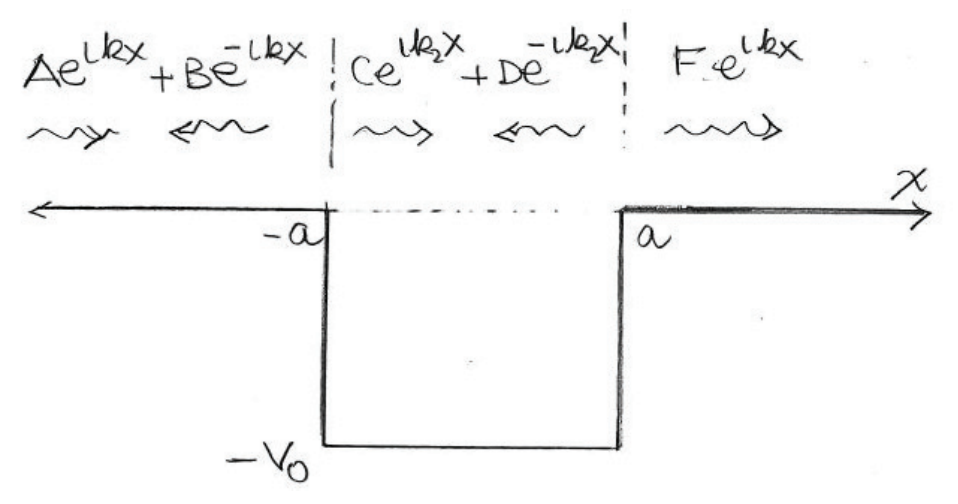
\includegraphics[width=0.5\linewidth]{resources/images/finite_square_well_scattering.png}
    \caption{Waves inside a finite square well.}
    \label{finite_square_well_scattering}
\end{figure}

Here $A$ is the coefficient of the incoming wave and $B$ is the coefficient of the reflected wave. Both of these waves have wavenumber $k$. In the well, there is a well moving to the right with coefficient $C$ and a wave moving to the left with coefficient $D$; both of these waves have wavenumber $k_2$. To the right of the well we have just one wave with coefficient $F$ moving to the right with wavenumber $k$. 

\begin{framedrmk*}[Symmetry breaking]
    Note that even though the potential is even, Corollary \ref{even_potential_cor} applies only to \textit{bound} states. Notably, the scattering states do not have to be even or odd. The symmetry is broken by the condition that the wave is incident from the left.
\end{framedrmk*}

\begin{framedrmk*}[Reflecting on a potential dip]
    In quantum mechanics, \textit{any} change in the potential can cause a reflection. This is the cause of the $B$ wave in Figure \ref{finite_square_well_scattering}; the incoming wave reflects off the potential dip at $x=-a$. This is similar to a string wave that encounters a change in the density of the string --- in general, there will always be a reflected and a transmitted component.
\end{framedrmk*}

The values of $k$ and $k_2$ are determined by the Schrödinger equation: $$k^2=\frac{2mE}{\hbar^2},\quad k_2^2=\frac{2m(E+V_0)}{\hbar^2}.$$There are four boundary conditions, given by continuity of $\psi$ and $\psi'$ at $x=-a$ and $x=a$. These four equations can be used to fix the coefficients $B$, $C$, $D$, and $F$ in terms of $A$. Since the outgoing waves to the left and right have the same wavenumber as the incoming wave, we define reflection and transmission coefficients $R$ and $T$ as $$R=\frac{|B|^2}{|A|^2},\quad T=\frac{|F|^2}{|A|^2}.$$From Theorem \ref{current_conservation_thm}, we know that the probability currents to the left and right of the well must be equal: $$|A|^2-|B|^2=|F|^2.$$Rearranging, $$\frac{|B|^2}{|A|^2}+\frac{|F|^2}{|A|^2}=R+T=1.$$

\subsection{Resonant Transmission}\label{resonant_transmission}

Solving for $R$ and $T$ is straightforward but a little tedious, so we will just quote the answer. The transmission coefficient is given by the following relation: $$\frac{1}{T}=1+\frac{1}{4}\frac{V_0^2}{E(E+V_0)}\sin^2(2k_2a).$$Since the second term is always positive, we have $T\leq 1$. As $E\to 0$, we have $\frac{1}{T}\to\infty$, so $T\to 0$. Also, as $E\to\infty$, we have $T\to 0$. Additionally, there is the possibility that $T=1$ if $\sin(2k_2a)=0$. This is called \textbf{resonant transmission}.

We can remove all units from this result by defining $$e=\frac{E}{V_0},\quad z_0^2=\frac{2ma^2V_0}{\hbar^2}.$$Then $$(k_2a)^2=\frac{2ma^2(E+V_0)}{\hbar^2}=\frac{2ma^2V_0}{\hbar^2}(1+e),$$so $$2k_2a=2z_0\sqrt{1+e}.$$We can similarly rewrite the $\frac{V_0^2}{E(E+V_0)}$ factor in terms of $e$. We get $$\boxed{\frac{1}{T}=1+\frac{1}{4e(1+e)}\sin^2(2z_0\sqrt{1+e}).}$$We now see that $T=1$ if $$2z_0\sqrt{1+e}=n\pi,\quad n\in\mathbb{Z}.$$Not all integers are allowed! Note that $e>0$ since the energy is positive. Thus, the left-hand side is at least $2z_0$, so $$n\geq \frac{2z_0}{\pi}.$$Let the associated energies be $E_n=e_nV_0$. Then $$e_n+1=\frac{n^2\pi^2}{4z_0^2}=\frac{n^2\pi^2\hbar^2}{2m(2a)^2V_0}.$$Multiplying both sides by $V_0$, we have $$E_n+V_0=\frac{n^2\pi^2\hbar^2}{2m(2a)^2}.$$Note that $E_n+V_0$ is the energy of the scattering state measured from the bottom of the finite square well. The right-hand side is the energy of the $n$th bound state of the \textit{infinite} square well of width $2a$, as shown in Figure \ref{resonant_transmission_well}. We thus have the following (rather surprising) result.

\begin{framedthm}[Resonant transmission in the finite square well]
    Resonant transmission in a finite square well occurs for those energies $E_n>0$ that are in the spectrum of the infinite square with the same width as our finite square well.
\end{framedthm}

\begin{figure}
    \centering
    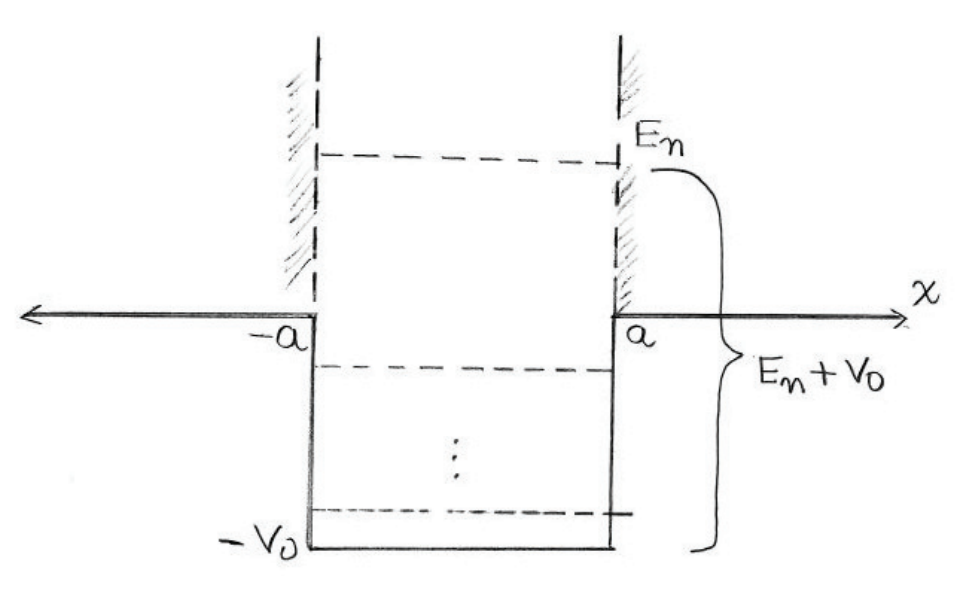
\includegraphics[width=0.5\linewidth]{resources/images/resonant_transmission_well.png}
    \caption{The energy levels for which resonant transmission occurs in the finite square well are precisely the energy levels of an equally-wide infinite square well.}
    \label{resonant_transmission_well}
\end{figure}

Since infinite square well bound states are characterized by fitting an integer number of half wavelengths inside the well, we have resonant transmission when the scattering waves fit perfectly inside the finite square well. This can also be seen directly from the vanishing of $\sin (k_2(2a))$ in the expression for $\frac{1}{T}$.

\begin{framedexpl}[Transmission coefficient for a given well]
    Figure \ref{resonant_transmission_example} depicts the transmission coefficient as a function of $e=E/V_0$ for a finite square well with $z_0=13\pi/4$. In this case, we must have $n\geq 7$. Notice that $T$ broadly approaches $1$ but only ever reaches it for discrete energy values.
\end{framedexpl}

\begin{figure}
    \centering
    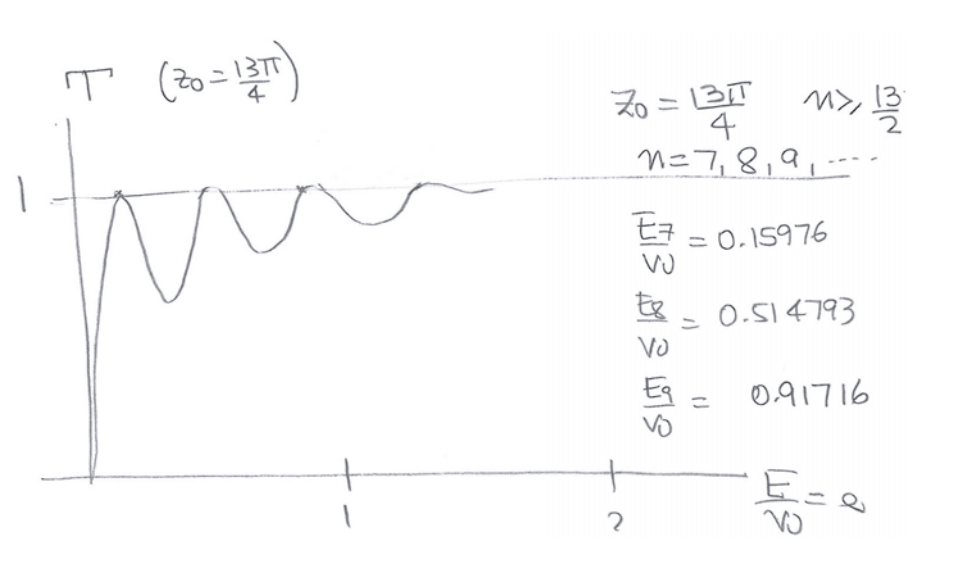
\includegraphics[width=0.65\linewidth]{resources/images/resonant_transmission_example.png}
    \caption{A graph of the transmission coefficient as a function of energy in a finite square well.}
    \label{resonant_transmission_example}
\end{figure}

\subsection{The Ramsauer-Townsend Effect}\label{ramsauer_townsend}

In 1921, Carl Ramsauer and John Sealy Townsend were studying the elastic scattering of low-energy electrons off of noble gas atoms. These gases have their electron shells fully filled and are both very un-reactive and have high ionization energies. 

Since the atom is electrically neutral, there is no potential far away from the atom. However, as the incident electron passes through the outer electron shell the potential due to this shell becomes $0$ by the Shell Theorem. The incident electron then experiences a spherically-symmetric attractive potential due to the nucleus-- some kind of finite spherical well. In the experiment, some electrons collided with the nuclei of the atoms and scattered, most bouncing back. Thus, we can view the reflection coefficient $R$ as a proxy for the scattering cross-section. 

Ramsauer and Townsend reported a very strange phenomenon. At very low energies, the scattering cross section was high. But as the energy was increased, the scattering went to $0$, and for it to go up again, the energy had to increase further. This behavior had no sensible classical explanation. 

In fact, this was an early example of quantum-mechanical resonant transmission. The reflection coefficient approaching $0$ meant the transmission coefficient going to $1$, which we know occurs for discrete values of $E$. Figure \ref{reflection_transmission_coefficients} displays both $R$ and $T$ as a function of energy. At the arrow, we have $R=0$, so there is no scattering. All of the electrons go straight through the atoms!

\begin{figure}
    \centering
    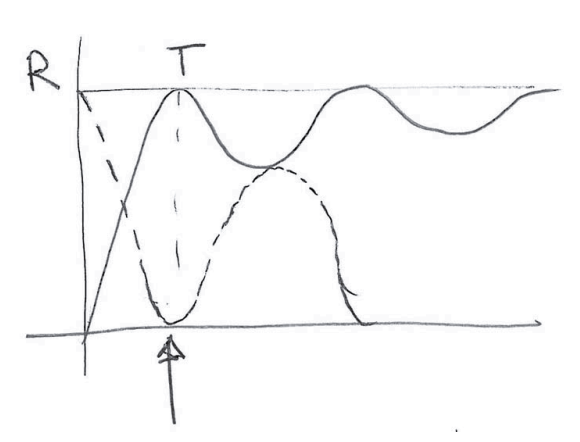
\includegraphics[width=0.5\linewidth]{resources/images/reflection_transmission_coeffs.png}
    \caption{A graph of the reflection coefficient $R$ and the transmission coefficient $T$ with respect to energy.}
  \label{reflection_transmission_coeffs}
\end{figure}